\documentclass[a4paper, amsfonts, amssymb, amsmath, reprint, showkeys, nofootinbib, twoside]{revtex4-1}

\usepackage[english]{babel}
\usepackage[utf8]{inputenc}
\usepackage[colorinlistoftodos, color=green!40, prependcaption]{todonotes}
\usepackage{graphicx}
\usepackage{subcaption}
\usepackage{float}
\usepackage[bottom]{footmisc}
\usepackage{enumitem}
\usepackage{hyperref}

\bibliographystyle{apsrev4-1}
\setlist{noitemsep}

\begin{document}

\title{%
  \large{Vipassana for Hackers} \\
  \Huge{Paper Two: The Brain} \\
  \large\textit{Version 0.3}
}
\author{Preethi Govindarajan}
\email[Correspondence email address: ]{preethi@deobald.ca}
\affiliation{Siggu.org}
\date{\today}

\begin{abstract}
  Two years ago, immediately following my first Vipassana course, I began researching
the effects of meditation on the brain. This paper is a summary of the research
available on the topic and speculations, based on my experience, as to what is
happening in the brain during a 10-day silent Vipassana meditation retreat.
\end{abstract}

\keywords{neuroscience, vipassana, meditation}

\maketitle

% \listoftodos

\section{Introduction}

I took my first Vipassana course (as taught by S.N. Goenka) in 2017.
Vipassana meditation was so unlike anything I had ever experienced before
I was left extremely curious about what exactly had happened
to me during those ten days. For months afterward I spent my mornings and
evenings wading through the research in the field of meditation. I was specifically
focused on white papers dealing with the effects of a 10-day Vipassana course on
the brains of participants. The research in this area is limited.
The quality research which does exist usually uses a sample of highly
experienced meditators \cite{tibetanmonks} rather than beginners and/or self-reports rather than
objective measures.

Over the past year, I have tried to write down what I experienced during that first
10-day course and the 10-day courses I have taken since, corroborating my experience
with research that does exist regarding meditation and the brain.

\textbf{Proviso:} S.N. Goenka, the principal teacher of Vipassana meditation,
actively dissuades students from precisely the sort of brain-centred biological
inquiry presented in this paper.

\begin{quote}
  \textbf{The brain itself is just a physical organ. As you deal with other parts of
    the body, you deal with the brain in the same way, that's all. Nothing special to
    do with the brain. But the mind is totally different. In the West, all importance
    is given to the brain as if the mind is located here. Nothing doing, it is
    everywhere. The mind is in the whole body. So give attention to the whole
    body.} --- S.N. Goenka \cite{goenkabrain}
\end{quote}

This paper does not contradict Mr. Goenka's sentiment, but instead acts as a starting
point for curious readers who, whether they have taken a Vipassana course or not,
view the function of the brain as central to the activity of the mind.

\textbf{Disclaimer:} Although my primary field of research is within the field of
biology, my work is far removed from neuroscience. I have tried to simplify the research available so as to better
understand it. If there are any corrections to make or editing in terms of the
content, please feel free to contact me.


\section{Brain Function and Anatomy}

Before dissecting the experience of meditation as it pertains to the brain, this
section describes the different parts of the brain that have shown up in
scientific literature as correlated to meditative practices. Recent neuroscience divides the
brain into the reified geography of the brain (anatomy) and the abstract concepts
governed by brain activity (function). Between concrete physiology and abstract
functional outcomes exist networks of cooperative structures which correspond to general
high-level activities of the brain.

The Default Mode Network (DMN) is the constellation of regions which fire when
the brain is not engaged in any external or goal-oriented
tasks. As the name suggests, the brain is in its ``default
mode'' of operation. \cite{defaultnetworkadaptive} The DMN is anticorrelated to the Central Executive
Network (CEN), which is active during externally-directed, high-level cognitive
functions. \cite{saliencenetwork} This anticorrelation between the DMN and the CEN is
governed by the Salience Network (SN), the collection of regions in the brain which
help decide which stimuli deserve our attention. In this way, the SN acts as a switch between the
internally-directed DMN and the externally-directed CEN. \cite{saliencenetwork}

Where possible in the following sections these networks are described in terms of
function. The description of the DMN is also organized by function but the subsystems
of the CEN and SN offer too many potential functional categorizations and are instead
organized by anatomy.

\begin{figure}[H]
  \centering
  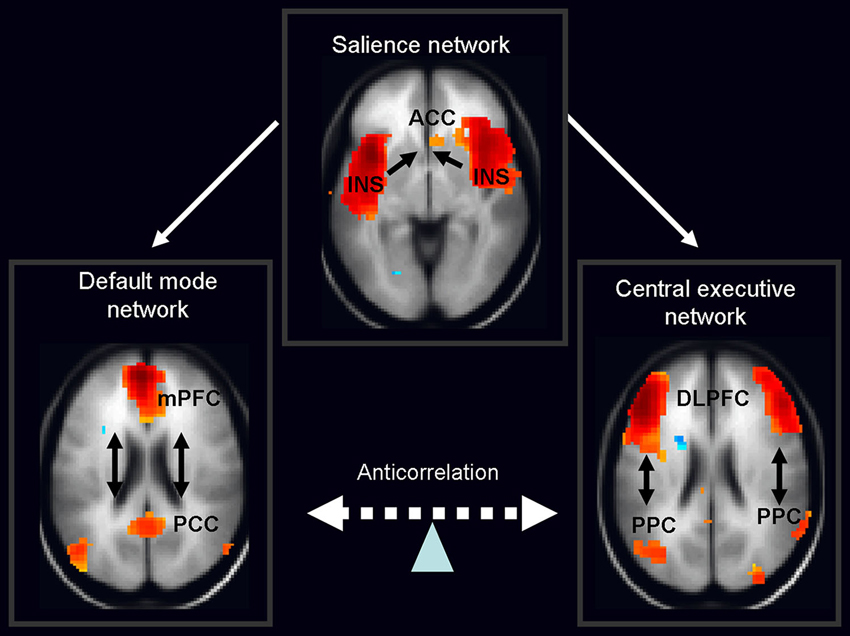
\includegraphics[width=7.5cm]{images/fmri-switching.jpg}
  \caption{The Salience Network consists of the Anterior Cingulate Cortex and the
    Anterior Insular Cortex. It helps switch between the Default Mode Network and the
  Central Executive Network.}
  \label{fig:fmri-switching}
\end{figure}

\subsection{Default Mode Network}

The DMN is comprised of specific anatomy including portions of the mid-line of the
brain, an evolutionarily primitive area related to memory and emotion, and
structures in the cortex, an evolutionarily recent part of the brain containing the
executive and higher order functions. \cite{defaultnetworkanatomy}

These functionally connected regions are involved in the neurological basis
of the self, considering the mental states of others, remembering the past, and
imagining the future.

This network is mostly observed through changes in blood flow to different parts of
the brain measured using fMRI (functional Magnetic Resonance Imaging) or
PET (Positron Emission Tomography). \cite{defaultnetworkadaptive}

\begin{figure}[h!]
  \centering
  \begin{subfigure}[b]{0.48\linewidth}
    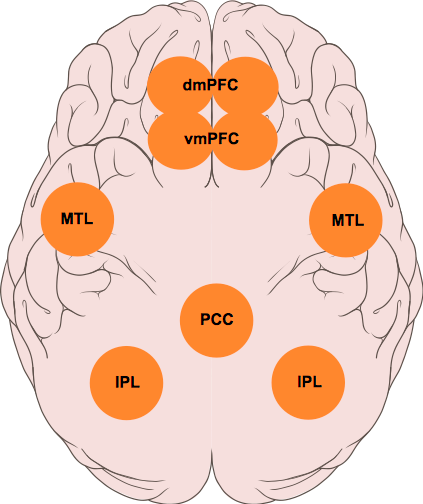
\includegraphics[width=\linewidth]{images/top-dmn.png}
  \end{subfigure}
  \begin{subfigure}[b]{0.48\linewidth}
    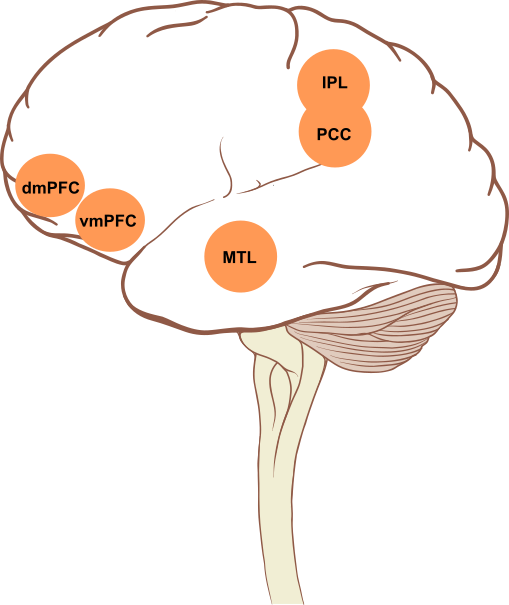
\includegraphics[width=\linewidth]{images/side-dmn.png}
  \end{subfigure}
  \caption{Highlighted: approximate locations of brain regions firing when the Default Mode Network is active.}
  \label{fig:dmn}
\end{figure}

\subsubsection{The neurological basis of the self}

The regions involved in an individual's conceptual ``self'' are the Posterior
Cingulate Cortex (PCC), Ventromedial Prefrontal Cortex (vmPFC), and the Inferior
Parietal Lobule (IPL). Observationally, these regions are preferentially activated when
subjects were asked to reflect on personal preferences, beliefs, abilities, or
any other qualities relevant to the self. \cite{defaultnetworkadaptive} Cerebral
blood flow and metabolic rate are 40\% higher than average in the PCC,
making it one of the most active regions of the brain. \cite{pccrole}

The PCC has been thought to mediate interactions between emotion and memory.
Under an fMRI, it consistently lights up when a person recollects an event from their
life. The strength of this activity varies depending on the emotional importance of
the memory recalled. It is also activated by emotional stimuli,
both positive and negative, and acts as a navigational interface, between the individual
and the external world, by gauging the importance of different stimuli. \cite{pccemotion}

The vmPFC is involved in creating a conceptual self by self-related processing
and the assignment of personal significance to self-related
information. \cite{dmnself} The vmPFC is paired with the Dorsomedial Prefrontal
Cortex (dmPFC), which assists in the creation of the conceptual self through an
individual's consideration of ``others''. Together, the vmPFC and dmPFC form the
Medial Prefrontal Cortex (mPFC).

The Inferior Parietal lobe (IPL) is situated in the back of the brain and it is
involved in the perception of facial stimuli. \cite{ipl}
The IPL has been hypothesized as being involved in distinguishing self from others,
in a study where subjects were asked to retrieve
previous judgments about oneself, their friend and the Dutch queen,
the activation of the IPL was seen to decrease with decreasing self-reference. \cite{iplself}
Another study also used Transcranial Magnetic Stimulation (TMS) to create a sort of "virtual lesion"
(transiently disturb the neural circuitry in that area) of
the right-IPL and showed that this disrupts self-other discrimination. \cite{ipltms}

It is hypothesized that the activation of these three regions of the brain (PCC,
vmPFC, and IPL) are responsible for providing a sense of self --- a subjective agent
in space and time. It functions as a network in which phenomena such as self
representations are accessible via the PCC \cite{mappingself} and are gated into
conscious awareness by activity in the mPFC, as influenced by changing internal
and external demands. The PCC acts as a brain-wide connectivity hub, through which a unitary notion of self is
created by a large scale integration of DMN activity. \cite{mappingself}

\subsubsection{Thinking about others}

The \textit{Theory of Mind} is a body of work in philosophy and psychology which
describes an individual's ability to consider the mental states of others, such as
appreciating another individual's false beliefs (knowledge based on incorrect or
outdated information). The Theory of Mind captures not only one's ability to
attribute beliefs, desires, and emotions to others but also to oneself --- and to
differentiate the two. \cite{autistictheoryofmind}

The DMN (especially the dmPFC subsystem) is engaged when individuals reflect upon,
evaluate, or appraise their own mental states or the mental states of others. ``Mental
states'' include thoughts, feelings, and desires. \cite{theoryofmind} In addition to
consideration of these states, the dmPFC is involved in empathy, moral reasoning,
and altruistic behavior. \cite{defaultnetworkadaptive,dmpfcothers,dmpfcaltruism}

\begin{figure}[H]
  \centering
  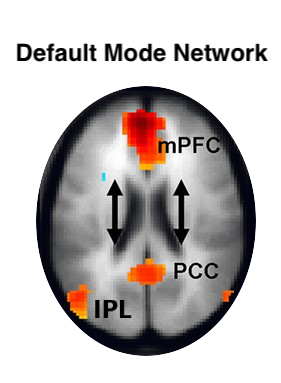
\includegraphics[width=5cm]{images/fmri-dmn.png}
  \caption{fMRI scan of the Default Mode Network.}
  \label{fig:fmri-dmn}
\end{figure}

\subsubsection{Autobiographical memory and future simulations}

The term "autobiographical memory" refers to our memory for specific episodes,
and to our conceptual, generic, and schematic knowledge of our lives.

The Medial Temporal Lobe (MTL) which is found on the medial surface of the temporal lobe.
The critical role of the MTL in long term memory is well documented. \cite{mtl}

The MTL consists of the hippocampal formation on top and the parahippocampal gyrus below it as well as
the entorhinal and perirhinal cortices.
The MTL, amygdala, the olfactory cortex, hypothalamus and several other
anatomically connected areas forms the limbic system. It appears to be primarily responsible for
our emotional life and has a specific involvement in the formation of memories. \cite{limbic}

The MTL along with mPFC, IPL and PCC forms the Medial Temporal Subsystem (a part of the DMN).
This subsystem is triggered during autobiographical memory retrieval,
contextual association, and semantic knowledge. \cite{defaultnetworkadaptive}

It has been hypothesized that the adaptive role of memory retrieval is to facilitate
construction of episodes to prepare for immediate and distant future scenarios. \cite{defaultnetworkadaptive}
The DMN is therefore involved in remembering the past, imagining the future, and story
comprehension. \cite{defaultnetworkadaptive}

\subsubsection{Summary}

The DMN plays a role in constructing a sense of self, in memory,
and in thinking about others. Because of this, it is also a key component in excessive
rumination and anxiety. \cite{dmndepression}

When a meditator sits down to meditate and thoughts wander away to past experiences
or anxieties about the future, classic meditation texts and instructions refer to
this behaviour as ``Monkey Mind''. It is the DMN playing the most active role in this
distraction.

\subsection{Central Executive Network}

The CEN is activated when high-level cognitive tasks or external goal-oriented tasks
are being performed. These tasks or executive functions are cognitive processes involved in
cognitive control of behavior. This depends on three types of brain functions:
working memory, mental flexibility, and self-control. The regions of the brain
involved in these executive functions are the Dorsolateral Prefrontal Cortex
(DL-PFC), Orbito Frontal Cortex (OFC), and the Posterior Parietal Cortex (PPC).

\begin{figure}[h!]
  \centering
  \begin{subfigure}[b]{0.48\linewidth}
    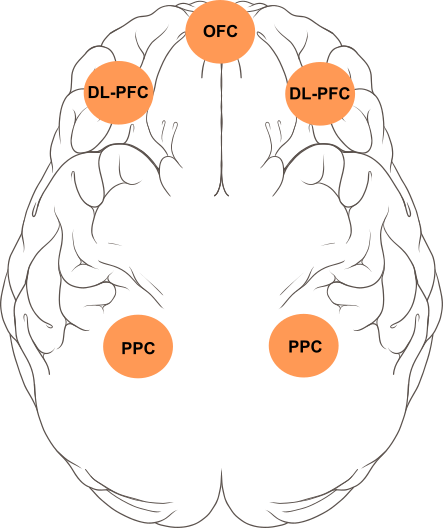
\includegraphics[width=\linewidth]{images/top-cen.png}
  \end{subfigure}
  \begin{subfigure}[b]{0.48\linewidth}
    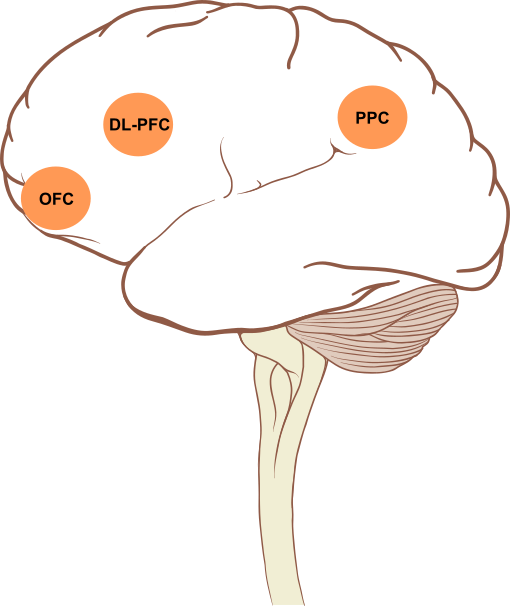
\includegraphics[width=\linewidth]{images/side-cen.png}
  \end{subfigure}
  \caption{Highlighted: approximate locations of brain regions firing when the Central Executive Network is active.}
  \label{fig:cen}
\end{figure}

\subsubsection{Dorsolateral Prefrontal Cortex}

The DL-PFC is a part of the Prefrontal Cortex found in primates, including
humans. The DL-PFC is involved in higher cognitive processes including working memory
(holding different pieces of information, manipulating them, and using them for
tasks), selective attention, cognitive flexibility (switching between tasks) and
planning. It also seems to be involved in social cognition and lying. The DL-PFC has
also been seen to increase dopamine levels in the brain. \cite{dlpfcmemory,dlpfctasks,dlpfclying}

\subsubsection{Orbito Frontal Cortex}

The OFC is an area found in front of both hemispheres of the brain, just above the
eyes. It is again a part of the Prefrontal Cortex and is thought to be involved in
decision making through emotion and reward. It also receives input from multiple
sensory modalities and in turn activates the Amygdala and the
Hypothalamus. \cite{theprefrontalcortex,ofcprimates,theorbitofrontalcortex}

\subsubsection{Posterior Parietal Cortex}
The PPC is a region of the Parietal Cortex, physically located behind the primary
Somatosensory Cortex. The PPC is responsible for facilitating higher-order
functions. Higher-order functions are defined as those requiring diverse information
for the purposes of higher evolutionary behaviour: intelligence, memory, planning,
speech, orientation, decision-making, etc.

To do this, the PPC receives input from auditory, visual, and somatosensory
systems, integrates this input, and uses the aggregate to activate the DL-PFC and motor cortex and is
involved in the performance of attention related tasks as well as higher-order motor
tasks such as grasping and catching. \cite{parietallobes}

\subsubsection{Sidenote: Somatosensory Cortex}
The Primary Somatosensory Cortex is located in a ridge of cortex found within the Parietal Cortex.
It is responsible for processing somatic sensations. These sensations arise from receptors
positioned throughout the body. They are responsible for detecting touch, for proprioception
(the position of the body in space), nociception (pain), and temperature. \cite{somato}
When such receptors detect one of these sensations, the information is sent first to
the Thalamus and then to the Primary Somatosensory Cortex.

The Sensory Homunculus which is a part of the Somatosensory Cortex is a cortical representation
of the body based on the degree of sensory innervation. \cite{sensoryhom}

\begin{figure}[H]
  \centering
  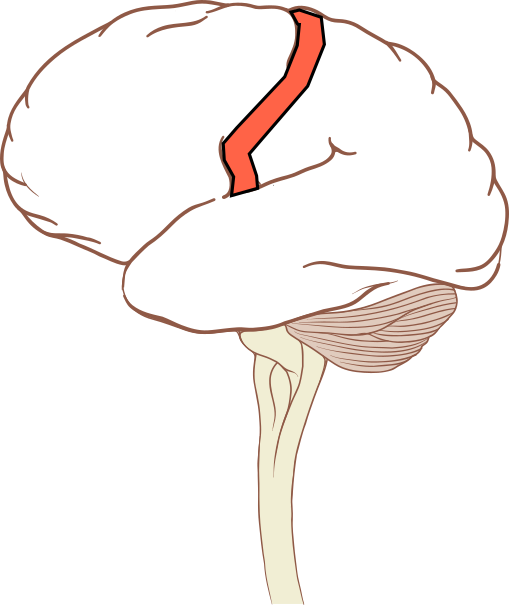
\includegraphics[width=5cm]{images/side-somatosensory.png}
  \caption{Location of the Somatosensory Cortex.}
  \label{fig:side-somatosensory}
\end{figure}

\begin{figure}[H]
  \centering
  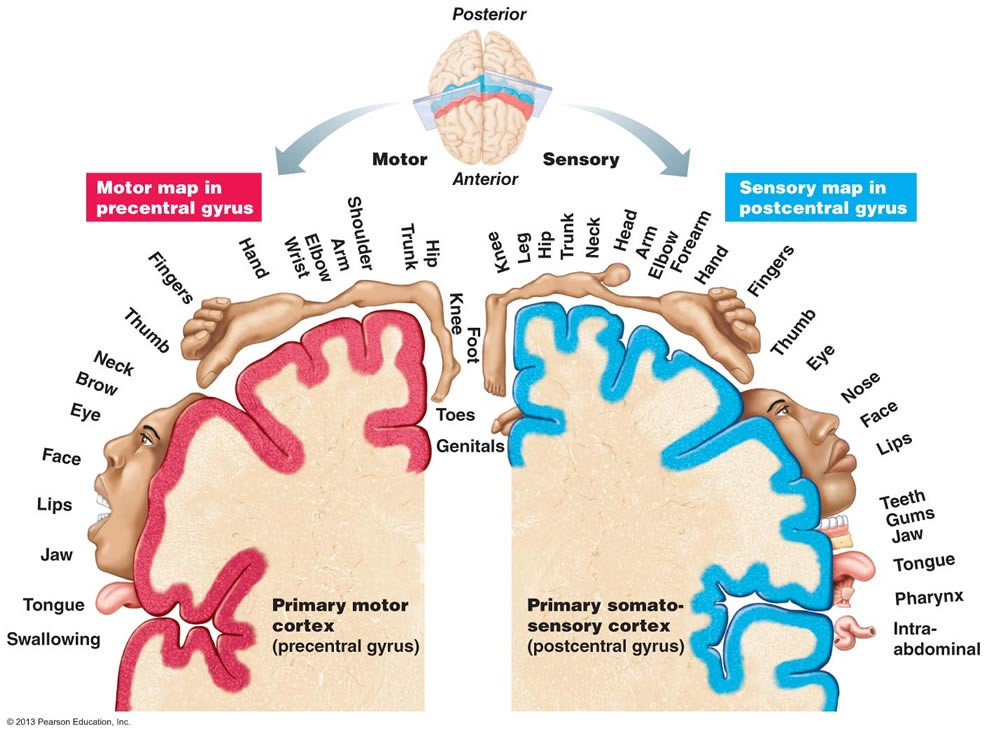
\includegraphics[width=7.5cm]{images/homunculus.jpg}
  \caption{The Sensory Homunculus mapped across the Somatosensory Cortex.}
  \label{fig:homunculus}
\end{figure}

\begin{figure}[H]
  \centering
  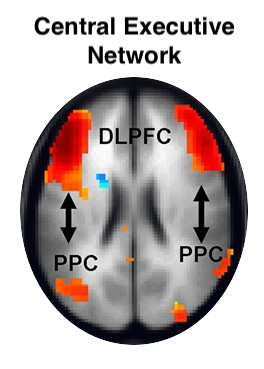
\includegraphics[width=5cm]{images/fmri-cen.png}
  \caption{fMRI scan of the Central Executive Network.}
  \label{fig:fmri-cen}
\end{figure}

\subsubsection{Summary}

The CEN is involved in goal-directed behavior and processes
related to attention. These goals are usually external and attention is also directed
externally (regardless of whether attention is voluntary or not). When you meditate,
attention is directed both internally and voluntarily, to the same sensory cues that
are normally directing the PPC.

\subsection{Salience Network}

\begin{quote}
  \textbf{Salience: The perceptual quality by which an observable thing stands out
    relative to its environment.}
\end{quote}

The SN is an intrinsically connected large-scale network anchored in the Anterior
Insular Cortex (AIC) and Dorsal Anterior Cingulate Cortex (ACC). Both regions have reached a
high degree of specialization in the great apes. It is the collection of the regions
in the brain that help decide which stimuli deserves our attention. It acts as a
switch between the internally-directed DMN and the externally-directed CEN. \cite{saliencenetwork}

\begin{figure}[h!]
  \centering
  \begin{subfigure}[b]{0.48\linewidth}
    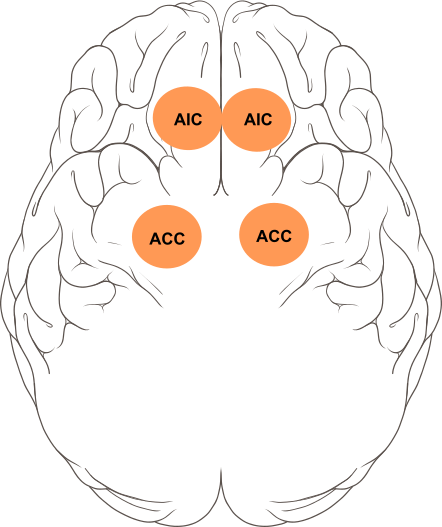
\includegraphics[width=\linewidth]{images/top-sn.png}
  \end{subfigure}
  \begin{subfigure}[b]{0.48\linewidth}
    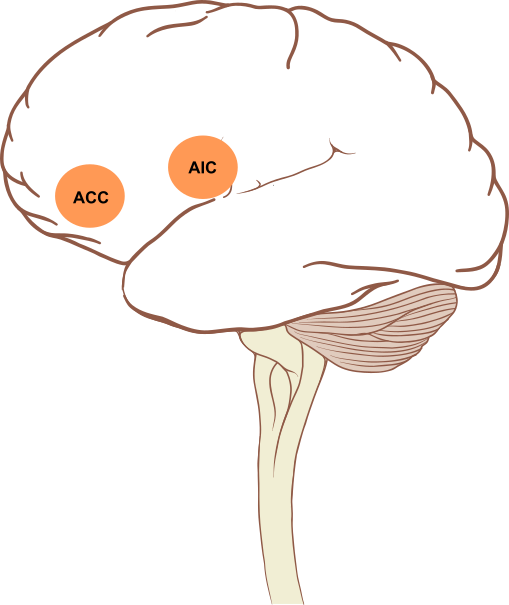
\includegraphics[width=\linewidth]{images/side-sn.png}
  \end{subfigure}
  \caption{Highlighted: approximate locations of brain regions firing when the Salience Network is active.}
  \label{fig:sn}
\end{figure}

\subsubsection{Anterior Cingulate Cortex}

The ACC is the front end of the Cingulate Cortex and collars around the Corpus
Callosum, the band connecting the two hemispheres of the brain. It is the connector
between the emotional (Limbic System) and the cognitive (Prefrontal Cortex) part of
the brain. It is involved in functions such as attention allocation, reward
anticipation, decision making, morality, impulse control, emotional awareness and
registering pain. \cite{accstroop,accreward,snmorality,empathypain,acccognitive} It
also appears to play a role in the regulation of Autonomic functions such as blood
pressure and heart rate. \cite{accbloodpressure}

\subsubsection{Anterior Insular Cortex}

The AIC is a part of the Cerebral Cortex located deep within the Sulcus, the
fissure separating the four lobes of the brain. The AIC physically projects itself
into the Amygdala. It is involved in multimodal sensory processing such as
audio-visual integration tasks, interoceptive awareness (so its activity is directly
related to an individual's sense of internal body states), empathy, and conscious
awareness. \cite{aicemotion}

It also plays a role in the regulation of autonomic functions such as bodily
sensations (including judgement of the severity of pain), taste, and control of the
immune system. \cite{aicautonomic}

The AIC and ACC together give rise to our interoceptive and conscious
self-awareness.  \cite{selfaware}

\begin{figure}[H]
  \centering
  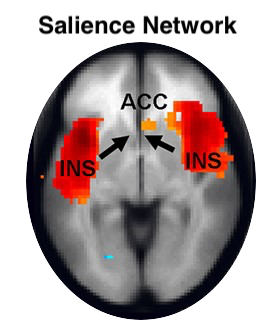
\includegraphics[width=5cm]{images/fmri-sn.png}
  \caption{fMRI scan of the Salience Network.}
  \label{fig:fmri-sn}
\end{figure}

\subsubsection{Summary}

The SN is directly involved in switching between the DMN and CEN. When you meditate,
you cultivate the cognitive processes related to attention.
When the meditator's mind wanders, she notices it and brings it back.
The SN is directly involved in this process of assigning attention, since it is
responsible for the prominence of any object of attention.
Meditation, or the act of returning to an object of meditation, can therefore be
thought of as an exercise in strengthening the SN and its ability to perform this switch, over time.


\section{The Course}

I applied for my first 10-day Vipassana course after I quit my job. From the time I
was accepted into the course until the first day of the course I was very nervous
about what it might entail. I had never done anything like meditation before
and I was quite happy with the idea that meditation, with its spiritual connotations
and religious mumbo-jumbo, was a waste of my time. In my mind, a silent meditation retreat was
for people who had time to waste --- and I was not one of them. Yet friends had convinced me that I
should give Vipassana a try and in the interval between workplaces I had
time to experiment with a course.

The following are my observations and speculations about what could be happening
in the brain during a 10-day course.

I went for my first course in Chennai, my home town. When I arrived, I had to fill
the application forms all over again (despite applying online), keep all my
luggage in a locker, and go to my room. I had to share the room with one other
student. I felt quite out of my element and I was certain everyone else could see
that I was the odd one out. In my head, I was not supposed to be there. Because I felt
so out of place, I was too scared to actually make conversation with anyone before
silence was enforced.

\subsection{Anapana Meditation}

And so it was. With my brain filled with thoughts about myself, about the people
around me, I started this meditation business. For the first 3.5 days I was instructed
to focus my attention on the area below my nostrils and above my upper
lip. That's all. These are undoubtedly very simple instructions but in practice I
found them very difficult. Maintaining my focus was much harder than I had
anticipated. Within the first two days, I had made up elaborate stories about my
fellow meditation students. In these fantasies all of the other students were
superheroes, tirelessly working to save humanity together. My Default Mode Network
was in overdrive.

Focusing our attention below the nostrils starts with observing breath --- coming in
and going out. As the teacher mentions in the late evening discourses, the reason for
starting with your breath is because this the only activity of the body which is both
conscious and unconscious --- it acts as a bridge to the unconscious mind and the
involuntary processes of the body.

There has been research in mice, showing a cluster of nerves called the
pre-Bötzinger Complex (preBötC), found in the brain stem of most mammals, which fires
with every breath taken. This breathing pacemaker seems to work not only for regular
conscious and unconscious breathing but for all kinds of breathing --- such as yawns,
sighs and gasps. The preBötC also appears to play a role in calming and
arousal. \cite{prebotcgeneration} It would be interesting to see the activation in
these neuron clusters during the first three days of a Vipassana course, even among
novice meditators.

During the meditation hours I was trying hard. I had decided that if I was to examine this practice
empirically, I had to give it an honest shot. I focused on the small patch beneath my
nostrils above my upper lip. Initially, while trying to observe one's breathing, the
mind will wander --- not just to fantasies of superheroes but to almost any object or
daydream imaginable --- as the mind wanders the Default Mode Network is working. With
the realization that the mind has wandered, and the consequent return of attention
back to the breath, the Salience Network is activated.
This happens slowly at first. One's mind wanders away for many, many minutes before
realizing that the object of attention, the breath, has been lost. But
at some point within the 3.5 days, the SN learns to bring attention back to the breath. After a few days, this
refocusing almost happens by habit, almost automatically.

As I gave in to this activity, tried to focus more intently, and tried to sit still for
longer continuous stretches of time, there were longer periods of awareness on that
patch of skin. With these longer periods of awareness came
stranger sensations arising and passing within that physical area. By the third day,
it felt like entire ecosystems were writhing and flopping and crashing, all of them
very alive in the area below my nostrils above my upper lip. Since Anapana meditation
is very simple and these strange sensations appeared within a few days of my practice
as an absolute beginner, it would be very interesting (and relatively easy) to study
the neurological and physiological basis for such sensations.

There have been studies that have shown that once subjects bring their
attention back to breath, the neural structures involved in the control
of the Autonomic Nervous System and attention start firing more actively
(in this case, the DL-PFC --- a part of the CEN, the Hippocampus --- a part of the
DMN, and the ACC --- a part of the SN). During Anapana there are also global
dampening changes seen in the brain, particularly within the DMN and the Amygdala, which is involved in
the flight-or-fight (stress) response. These changes have been
termed the ``relaxation response'', as they are antagonistic to the stress
response. This relaxation response can be thought of as a gateway to altered states
of mind. \cite{relaxationresponse}

\subsection{Vipassana Meditation}

After lunch on the fourth day the instructions for Vipassana are given. During
Vipassana, students transfer their attention from the patch below their nostrils to the top
of the head. From there, for two hours, instructions are given to slowly move
one's attention throughout the entire body: ``from the top of the head to the tips of
the toes.'' This movement of attention throughout the body is then repeated, over and
over. The two objectives while observing bodily sensations are focused attention (making
use of the narrow focus practiced during the Anapana period) and open monitoring
(observing the sensations objectively).

As this process progresses, the Salience Network (ACC and AIC) and some parts of
the Central Executive Network (DL-PFC, OFC, and PPC),
which are involved in the control of attention, fire more actively. The anti-correlation
between the DMN and CEN reduces. Usually when a person is engaged in an external task,
the OFC and PPC receive signals from all the sensory networks (Visual, Audio, Somatosensory, etc.) and,
in response, continuously send signals to the different motor cortices, Amygdala, and Hypothalamus to
respond by performing a task, feeling an emotion, etc.

But Vipassana is an internal task. The Salience Network is activated by focused
attention, which in turn activates the Central Executive Network. Rather than an
external task, as the CEN is accustomed to, the conscious instruction is to observe
bodily sensation --- and do nothing. So as you sit in silence with your eyes closed,
not moving your body physically but instead moving throughout your body with your
attention, the CEN is doing what it has always done. However, the outcomes of
activity in the CEN are different during Vipassana. Instead of focusing on
external sensory input the sensory input is internal (bodily sensations) and instead
of reacting to input by performing tasks or feeling emotions the goal is to not
react, to simply observe as objectively as possible.

This is hard at first, with the body involuntarily reacting by jerking and writhing
in involuntary response to the very act of observation. Initially, even awareness
itself has a jerky quality and it is hard to observe sensations consciously. There is also the
pain. This eclipses all other sensations. In my case, it was difficult to maintain
awareness of any other sensation with the pain that was emanating from my legs and
back. The OFC is involved in assigning emotion to sensation and the shaping of pain by expectations
\cite{ofcemotion,ofcexpect} and the ACC plays a vital role in perception of sensation.
These two parts of the brain are usually functionally connected.
In the beginning, as I sat trying to observe sensations and was only aware of the pain,
the ACC was firing rapidly and the OFC then assigned these signals to the Limbic System, which
put me in a less than ideal emotional state.

Over the final seven days of the course, as awareness gets smoother and observations get more objective, this
functional connectivity between the ACC and the OFC slowly starts changing. While
continuing to pay attention to constantly changing bodily sensations the goal remains: avoid
assigning evaluations (and therefore, emotions) to them. Without assigning an
emotional response, one learns to observe with a
non-judgmental attitude, particularly toward unpleasant stimuli. The ACC is still up-regulated
but the OFC and the Limbic System may acquiesce and, in turn, reactions become smaller and less
frequent. This snowball effect almost mirrors the spiral of brain behaviours
exhibited early in the course. Early in the course, the CEN's normal mode of
operation is in play, which is to experience unpleasant stimuli and react (desiring to rid the body of
them), which in turn causes the unpleasant stimuli to appear all the more
unpleasant. Once a measure of objectivity is reached, however, the brain's function
snowballs in the other direction. It is as if both conscious and unconscious awareness-es are slowly aligning
until there are occasions of experience when it feels as if there is nothing but detached awareness moving
through the body (or some parts of the body). This is not at all akin to the
detachment of sleep or intoxication, however, and the senses are not dulled. In
addition to a feeling of emotional detachment, the ACC, AIC and the Somatosensory
Cortex, which are involved in sensory awareness, were \textbf{more} active, not
less. As the OFC, and Limbic System are calmed and attention is narrowed
further, the sensations become progressively more intense.

Perhaps the strangest experience during a Vipassana course is that of shifts in the
sense of self. The ``self'', as a subjective agent in space and time, changes. At
first, this change is only very slight. As a student closes her eyes and begins to
meditate, it may feel as though the body has shifted in space or rotated in different direction, this is
due to the temporary down regulation of the prefrontal cortex. As the meditations get deeper the DMN
occasionally quiets completely (perhaps only for a short duration) while the AIC
fires more rapidly, leading to alternative networks of consciousness
arising.

Consciousness is defined as our subjective awareness of ourselves and our environment.
An altered state of consciousness is defined as alternate patterns or configurations of
this experience, which differ qualitatively from a baseline state.
Altered states of consciousness include a state of dreaming, epileptic seizures, sensory deprivation,
hysterical states of dissociation and depersonalization as well as pharmacologically induced altered states.

The notion of altered states of consciousness has been put forth another way by the
Entropic Brain Hypothesis, described by Robin Carhart-Harris et al, while studying
the brain under the influence of psychedelics. \cite{entropic,entropicrevisited} Entropy is a measure of the
uncertainty in a system and, in this case, applies
to states of consciousness and their associated neurodynamics. The theory makes a
distinction between
two fundamental modes of consciousness: Primitive Consciousness and the normal Secondary
Consciousness of waking states.
Primitive consciousness is characterized by higher entropy and it is hypothesized to have
preceded the development of modern, adult, human, normal waking consciousness.
It is argued that suppression of this entropy facilitates normal waking consciousness
and associated metacognitive functions such as reality-testing and self-awareness.

Even one ten-day course will expose a student to these altered states of
consciousness and provide access to Primitive Consciousness. However, unlike
psychedelics, the Vipassana student is not under the control of an external force. If
she opens her eyes and stops meditating, these disorienting altered states of
consciousness instantly disintegrate. Lasting changes to consciousness caused by
Vipassana take a different shape.

Sometimes it feels like loosening the hold of one's own narrative leads to new insights that are
usually kept from consciousness. It has been found that experiencing this, even for a
few seconds, can lead to lasting changes long after the activity of meditation itself
has stopped. \cite{alteredtraits} In the moment, these experiences can be quite
similar to the influence of certain hallucinogenic drugs or even, in some cases, to ecstatic
seizures where the abnormal activity of the Anterior Insular Cortex leads to
heightened self-awareness, feelings of bliss, and a lack of
ambiguity. \cite{cortexbliss} Outside the activity of meditation, the lasting effects
(``Altered Traits'') of meditation are not so extreme. They tend to include
heightened awareness, improved concentration, and increased empathy, among
others. \cite{alteredtraits}

\section{Conclusion}

I believe attending a 10-day Vipassana course did, in fact, change the habit pattern
of my mind --- at least for a while.

Vipassana causes global dampening changes in the DMN, causes certain parts of
the SN and CEN to activate. That is, reacting parts of the network and
portions of the network which are aware of bodily sensation, respectively.
This changes a person's behavior and these changes can often be seen as soon as
someone leaves the course on the tenth day.

But repeated practice is essential for any sustained neuroplasticity since rewriting
many years of habit formation requires more than a ten day course. However, the
10-day course is both progressive and systematic. It is designed to give someone
experimenting with meditation the minimum observational change necessary to instill
an interest, to keep practicing.

There have been studies looking at both the structural changes in the brain and
functional changes in brain activity, especially to the DMN and the SN. But such
studies are often only done on meditators who have clocked thousands of hours of
practice, which diverges from the purpose of this paper. \cite{tibetanmonks,
  experiencemed, experiencemeda}

How is Vipassana different from simply concentrating on a task, as hard as one can?
When concentrating on any task, your DMN is quieted, the SN and CEN are firing, and you
enter into a state of flow. But flow or no flow, the reacting part of the brain is
also working. The mind may learn to focus intensely but the habit patterns of the
mind are unlikely to change. The goal of Vipassana is not simply to concentrate or to
enter a state of flow, but to break old reactionary habit patterns altogether.

As I left the Vipassana Center, I was really intrigued as to what exactly had
occurred over those ten days. What was it that had changed in my brain? I had to
know. I very quickly noticed, however, that as I left the centre, those very changes
started slipping away. But with each hour-long meditation at home, a tiny bit sticks
just a little more. And I get closer to my answer.


\section*{Acknowledgements}

Thank you to Steven Deobald for reviews, edits, and corrections. \texttt{Brain\_human\_normal\_inferior\_view.svg} and
\texttt{Brain\_human\_lateral\_view.svg} by Patrick J. Lynch, medical illustrator, CC-BY 2.5 \cite{brainsvg}


\section*{References}

\begin{thebibliography}{99}

\bibitem{tibetanmonks}
  Alex Hankey
  \url{https://www.ncbi.nlm.nih.gov/pmc/articles/PMC1697747/}
  \textit{Studies of Advanced Stages of Meditation in the Tibetan
          Buddhist and Vedic Traditions. I: A Comparison of General Changes}
  Evid Based Complement Alternat Med. 2006 Dec; 3(4): 513–521.

\bibitem{goenkabrain}
  S.N. Goenka.
  \url{https://www.vridhamma.org/A-store-house-of-answers-by-Shri-S-N-Goenka}
  \textit{Answers by Mr. S. N. Goenka}

\bibitem{defaultnetworkadaptive}
  Andrews-Hanna, Jessica R.
  \textit{The brain’s default network and its adaptive role in internal mentation.}
  The Neuroscientist: A Review Journal Bringing Neurobiology, Neurology and
  Psychiatry. 18 (3): 251–270. doi:10.1177/1073858411403316. ISSN 1089–4098. PMC
  3553600. PMID 21677128. (2012–06–01).

\bibitem{defaultnetworkanatomy}
  Buckner, R. L.; Andrews-Hanna, Jessica R.; Schacter, D. L.
  \textit{The Brain's Default Network: Anatomy, Function, and Relevance to Disease.}
  Annals of the New York Academy of Sciences. 1124 (1): 1–38. CiteSeerX
  10.1.1.689.6903. doi:10.1196/annals.1440.011. PMID 18400922, 2008

\bibitem{saliencenetwork}
  Menon, V; Toga, A.
  \textit{Salience Network.}
  Elsevier. pp. 597–611, 2015
  ISBN: 978–0–12–397316–0.

\bibitem{pccrole}
  Leech R, Sharp DJ
  \textit{The role of the posterior cingulate cortex in cognition and disease.}
  Brain. 137 (Pt 1): 12–32., July 2013.

\bibitem{pccemotion}
  Maddock, Richard J.; Garrett, Amy S.; Buonocore, Michael H.
  \textit{Posterior cingulate cortex activation by emotional words: fMRI evidence from a
    valence decision task.}
  Human Brain Mapping. 18 (1): 30–41. January 2003.

\bibitem{dmnself}
  Andrews-Hanna, Jessica R.; Smallwood, Jonathan; Spreng, R. Nathan.
  \textit{The default network and self-generated thought: component processes,
    dynamic control, and clinical relevance.}
  Annals of the New York Academy of Sciences. 1316(1):
  29–52. doi:10.1111/nyas.12360. ISSN 1749–6632. PMC 4039623. PMID 24502540. 2014-05-01.

\bibitem{ipl}
 Radua J, Phillips ML, Russell T, Lawrence N, Marshall N, Kalidindi S, El-Hage W, McDonald C,
 Giampietro V, Brammer MJ, David AS, Surguladze SA.
 \textit{Neural response to specific components of fearful faces in healthy
  and schizophrenic adults.}
  Neuroimage. 2010 Jan 1;49(1):939-46. doi: 10.1016/j.neuroimage.2009.08.030.
  Epub 2009 Aug 20.
  \url{https://www.ncbi.nlm.nih.gov/pubmed/19699306}

\bibitem{iplself}
 Hans C. Lou, Bruce Luber, Michael Crupain, Julian P. Keenan, Markus Nowak,
 Troels W. Kjaer, Harold A. Sackeim, Sarah H. Lisanby
 \textit{Parietal cortex and representation of the mental Self}
  Proc Natl Acad Sci U S A. 2004 Apr 27; 101(17): 6827–6832.

\bibitem{ipltms}
 Lucina Q. Uddin, Istvan Molnar-Szakacs, Eran Zaidel, Marco Iacoboni
 \textit {rTMS to the right inferior parietal lobule disrupts self–other discrimination}
  Social Cognitive and Affective Neuroscience, Volume 1, Issue 1, June 2006,
  Pages 65–71, https://doi.org/10.1093/scan/nsl003

\bibitem{mappingself}
  Davey CG, Pujol J, Harrison BJ.
  \textit{Mapping the self in the brain’s default mode network.}
  Neuroimage. 132:390–397., 2016-05-15

\bibitem{autistictheoryofmind}
  Baron-Cohen, Simon; Leslie, Alan M.; Frith, Uta.
  \textit{Does the autistic child have a ``theory of mind''?.}
  Cognition. 21 (1): 37–46. doi:10.1016/0010-0277(85)90022-8. PMID
  2934210. Pdf. October 1985.

\bibitem{theoryofmind}
  Frank Van Overwalle
  \textit{A dissociation between social mentalizing and general reasoning}
  NeuroImage. Volume 54, Issue 2, 15 January 2011, Pages 1589-1599
  \url{https://www.sciencedirect.com/science/article/abs/pii/S1053811910012243}

\bibitem{limbic}
  Catani M, Dell'Acqua F, Thiebaut De Schotten M
  \textit{A revised limbic system model for memory, emotion and behaviour}
  Neuroscience and Biobehavioral Reviews. 37 (8): 1724–37.
  doi:10.1016/j.neubiorev.2013.07.001. PMID 23850593.

\bibitem{dmpfcothers}
  Isoda, M., \& Noritake, A.
  \textit{What makes the dorsomedial frontal cortex active
    during reading the mental states of others?.}
  Neural basis of social learning, social deciding, and other-regarding preferences,
  51. 2015.

\bibitem{dmpfcaltruism}
  Waytz, A., Zaki, J., \& Mitchell, J. P.
  \textit{Response of dorsomedial prefrontal cortex predicts altruistic behavior.}
  The Journal of Neuroscience, 32(22), 7646–7650. 2012.

\bibitem{mtl}
 Scoville WB, Milner B
 \textit{Loss of recent memory after bilateral hippocampal lesions.}
 J Neurol Neurosurg Psych,  1957;20:11–21.

\bibitem{dmndepression}
  J. Paul Hamilton, Madison Farmer, Phoebe Fogelman, and Ian H. Gotlib.
  \textit{Depressive Rumination, the Default-Mode Network,
          and the Dark Matter of Clinical Neuroscience}
  Biol Psychiatry. 2015 Aug 15; 78(4): 224–230. doi: 10.1016/j.biopsych.2015.02.020

\bibitem{accstroop}
  Pardo JV, Pardo PJ, Janer KW, Raichle ME.
  \textit{The anterior cingulate cortex mediates processing selection in the Stroop
    attentional conflict paradigm.}
  Proceedings of the National Academy of Sciences of the United States of
  America. 87 (1): 256–9. doi:10.1073/pnas.87.1.256. PMID 2296583. January 1990.

\bibitem{accreward}
  Bush G, Vogt BA, Holmes J, Dale AM, Greve D, Jenike MA, Rosen BR.
  \textit{Dorsal anterior cingulate cortex: a role in reward-based decision making.}
  Proceedings of the National Academy of Sciences of the United States of
  America. 99 (1): 523–8. doi:10.1073/pnas.012470999. PMC 117593. PMID
  11756669. January 2002.

\bibitem{snmorality}
  Sevinc G, Gurvit H, Spreng RN.
  \textit{Salience network engagement with the detection of morally laden
    information.}
  Social Cognitive and Affective Neuroscience. 12 (7):
  1118–1127. doi:10.1093/scan/nsx035. PMID 28338944. July 2017.

\bibitem{empathypain}
  Jackson PL, Brunet E, Meltzoff AN, Decety J.
  \textit{Empathy examined through the neural mechanisms involved in imagining how I
    feel versus how you feel pain.}
  Neuropsychologia. 44 (5): 752–61. doi:10.1016/j.neuropsychologia.2005.07.015. PMID
  16140345. 2006.

\bibitem{acccognitive}
  Bush G, Luu P, Posner MI.
  \textit{Cognitive and emotional influences in anterior cingulate cortex.}
  Trends in Cognitive Sciences. 4 (6):
  215–222. doi:10.1016/S1364–6613(00)01483–2. PMID 10827444. June 2000.

\bibitem{accbloodpressure}
  Gianaros PJ, Derbyshire SW, May JC, Siegle GJ, Gamalo MA, Jennings JR.
  \textit{Anterior cingulate activity correlates with blood pressure during
    stress.}
  Psychophysiology. 42(6):627–35. 2005.

\bibitem{aicemotion}
  Xiaosi Gu, Patrick R. Hof, Karl J. Friston, Jin Fan.
  \textit{Anterior Insular Cortex and Emotional Awareness.}
  J Comp Neurol. 521(15): 3371–3388. 2013-08-15.

\bibitem{aicautonomic}
  Rolls ET.
  \textit{Functions of the anterior insula in taste, autonomic, and related
    functions.}
  Brain Cogn. 110:4–19. December 2016.

\bibitem{selfaware}
  Anil K. Seth, Keisuke Suzuki, Hugo D. Critchley
  \textit {An Interoceptive Predictive Coding Model of Conscious Presence}
  Front Psychol. 2011; 2: 395.

\bibitem{dlpfcmemory}
  Barbey AK, Koenigs M, Grafman J.
  \textit{Dorsolateral prefrontal contributions to human working memory.}
  Cortex. 49 (5): 1195–1205. May 2013.

\bibitem{dlpfctasks}
  Monsell S.
  \textit{Task switching.}
  Trends in Cognitive Sciences. 7 (3):
  134–140. doi:10.1016/S1364–6613(03)00028–7. PMID 12639695. 2003.

\bibitem{dlpfclying}
  Ito, Ayahito; Abe, Nobuhito; Fujii, Toshikatsu; Hayashi, Akiko; Ueno, Aya;
  Mugikura, Shunji; Takahashi, Shoki; Mori, Etsuro.
  \textit{The contribution of the dorsolateral prefrontal cortex to the preparation
    for deception and truth-telling.}
  Brain Research. 1464: 43–52. doi:10.1016/j.brainres.2012.05.004. 2012.

\bibitem{theprefrontalcortex}
  Fuster, J.M.
  \textit{The Prefrontal Cortex}
  Raven Press, New York, 1997.

\bibitem{ofcprimates}
  Rolls, ET.
  \textit{Convergence of sensory systems in the orbitofrontal
    cortex in primates and brain design for emotion.}
  The Anatomical Record Part A: Discoveries in Molecular, Cellular, and Evolutionary
  Biology. 281 (1):1212–25. doi:10.1002/ar.a.20126. November 2004.

\bibitem{theorbitofrontalcortex}
  Price, Joseph L.
  \textit{Chapter 3: Connections of the orbital cortex.}
  Rauch, Scott L.; Zald, David H.
  The Orbitofrontal Cortex. p. 45.
  Oxford University Press, New York. 2006.

\bibitem{somato}
  Viaene A.N.
  \textit {synaptic properties of thalamic input to layers 2/3 and 4 of
              primary somatosensory and auditory cortices}
  Journal of Neurophysiology. 105 (1): 279–292.
  doi:10.1152/jn.00747.2010. PMC 3023380.

\bibitem{sensoryhom}
  Marieb E, Hoehn K.
  Human Anatomy and Physiology.
  7th Ed. 2007. Pearson Benjamin Cummings: San Francisco.

\bibitem{parietallobes}
  Caspers S, Amunts K, Zilles K.
  \textit {Posterior Parietal Cortex: Multimodal Association Cortex.}
   The Human Nervous System. 3rd ed. New York: Elsevier; 2012.

\bibitem{relaxationresponse}
  Lazar SW; Bush George; Gollub RL.; Fricchione, GL.; Khalsa G; Benson H.
  \textit{Functional brain mapping of the relaxation response and meditation.}
  Neuroreport. 11(7):1581–1585. 2000-05-15.

\bibitem{prebotcgeneration}
  J. Muñoz-Ortiz, E. Muñoz-Ortiz, L. López-Meraz, L. Beltran-Parrazal,
  C. Morgado-Valle.
  \textit{The pre-Bötzinger complex: Generation and modulation of respiratory rhythm}
  Neurología (English Edition), ISSN 2173–5808,
  https://doi.org/10.1016/j.nrleng.2018.05.006. 2018.

\bibitem{ofcemotion}
  Rempel-Clower, N. L.
  \textit{Role of Orbitofrontal Cortex Connections in Emotion.}
  Annals of the New York Academy of Sciences,
  1121:72–86. doi:10.1196/annals.1401.026. 2007.

\bibitem{ofcexpect}
 Lauren Y.Atlas, Tor D.Wager
 \textit{How expectations shape pain.}
  Neuroscience Letters,  520 (2):140-148, 29 June 2012.

\bibitem{alteredtraits}
  Goleman, Daniel; Davidson, Richard J.
  \textit{Altered Traits}
  ISBN: 9780399184390. September 2018.

\bibitem{cortexbliss}
  Picard, Fabienne.
  \textit{State of belief, subjective certainty and bliss as a product of cortical
          dysfunction}
  Cortex, Volume 49, Issue 9, Pages 2494–2500ISSN 0010 9452. 2013.
  \url{https://doi.org/10.1016/j.cortex.2013.01.006}.

\bibitem{experiencemed}
   Brewer JA, Worhunsky PD, Gray JR, Tang YY, Weber J, Kober H.
   \textit{Meditation experience is associated with differences in default mode
           network activity and connectivity.}
   Proc Natl Acad Sci U S A. 2011 Dec 13;108(50):20254-9.
   doi: 10.1073/pnas.1112029108.

\bibitem{experiencemeda}
  Zoran Josipovic, Ilan Dinstein, Jochen Weber, David J. Heeger
  \textit {Influence of meditation on anti-correlated networks in the brain}
  Frontiers in Human Neuroscience, 03 January 2012.
  \url{https://doi.org/10.3389/fnhum.2011.00183}

\bibitem{entropic}
  Robin L. Carhart-Harris, Robert Leech, Peter J. Hellyer, Murray Shanahan, Amanda
  Feilding, Enzo Tagliazucchi, Dante R. Chialvo and David Nutt
  \textit{The entropic brain: a theory of conscious states informed by neuroimaging
    research with psychedelic drugs}
  Frontiers in Human Neuroscience, 03 February 2014.
  \url{https://doi.org/10.3389/fnhum.2014.00020}

\bibitem{entropicrevisited}
  Carhart-Harris, Robin L.
  \textit{The entropic brain - revisited}
  NEUROPHARMACOLOGY, Vol: 142, Pages: 167-178, ISSN: 0028-3908, 2018.

\bibitem{brainsvg}
  Patrick J. Lynch
  \texttt{Brain\_human\_normal\_inferior\_view.svg} and \textit{Brain\_human\_lateral\_view.svg}
  CC-BY 2.5
  \url{https://commons.wikimedia.org/w/index.php?curid=1496651}
  \url{https://commons.wikimedia.org/w/index.php?curid=1496648}


\end{thebibliography}

% \appendix*
% \input{sections/appendix1.tex}

\end{document}
